\section{Pregunta 03 – Enliste y describa los tipos de TableSpace que existen en Oracle}
Ejecutamos el siguiente comando
\begin{minted}{sql}
    SELECT TABLESPACE_NAME ,CONTENTS FROM DBA_TABLESPACES
\end{minted}

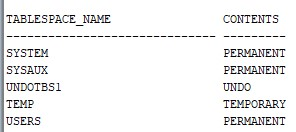
\includegraphics[width=8cm]{./images/tablespace}


\begin{enumerate}
    \item Permanente (PERMANENT) \\
Utiliza espacios de tabla permanentes para almacenar sus datos de usuario y aplicación. La base de datos Oracle utiliza espacios de tabla permanentes para almacenar datos permanentes, como los datos del sistema. A cada usuario se le asigna un espacio de tabla permanente predeterminado.

\item Deshacer (UNDO)\\

Una base de datos que se ejecuta en el modo de administración automática de deshacer crea y administra de forma transparente los datos de deshacer en el espacio de tablas de deshacer. La base de datos Oracle utiliza los datos de deshacer para revertir las transacciones, para proporcionar coherencia de lectura, para ayudar con la recuperación de la base de datos y para habilitar funciones como Oracle Flashback Query. Una instancia de base de datos solo puede tener un espacio de tablas de deshacer activo.

\item Temporal (TEMPORARY)\\

Los espacios de tabla temporales se utilizan para almacenar datos temporales, como se crearía cuando las sentencias de SQL realicen operaciones de clasificación. Una base de datos Oracle obtiene un espacio de tabla temporal cuando se crea la base de datos. Si estuviera creando un grupo de espacio de tablas temporal, crearía otro espacio de tabla temporal.
\end{enumerate}
